%/*% pdflatex -file-line-error -interaction nonstopmode %

\documentclass{article}
\usepackage{graphicx}
\graphicspath{ {./images/} }
\usepackage{amsmath}
\usepackage{amsfonts}
\usepackage{bookmark}
\usepackage{exercises}
\usepackage{amsthm}
\usepackage{yhmath}
\newcommand*{\oldneg}{\mathord{\sim}}

\theoremstyle{definition}
\newtheorem{definition}{Definition}

\setlength{\parindent}{.5in}
\setlength{\parskip}{12pt}

\title{1.7 Exercises}
\begin{document}
\maketitle

\section*{1}
A binomial is the sum of two monomials, while a trinomial is the sum of three monomials.

\section*{2}
Completing the square is a process to convert a binomial of the form $x^2+bx$ into a trinomial that can be factored using the perfect square trinomial 
pattern. This is accomplished by adding $\frac{b}{2}^2$ to the above binomial, as $x^2+bx+\frac{b}{2}^2$ is a perfect square trinomial.

\section*{3}
$x^2+4x+4=9\newline\rightarrow (x+2)^2=9\newline\rightarrow x+2=\pm 3\newline\rightarrow x=2\pm 3$

\section*{4}
$x^2+10x+25=64\newline\rightarrow (x+5)^2=64\newline\rightarrow x+5=\pm 8\newline\rightarrow x=-5\pm 8$

\section*{5}
$n^2+16n+64=36\newline\rightarrow (n+8)^2=36\newline\rightarrow n+8=\pm 6\newline\rightarrow n=-8\pm 6$

\section*{6}
$m^2-2m+1=144\newline\rightarrow (m-1)^2=144\newline\rightarrow m-1=\pm 12\newline\rightarrow m=1\pm 12$

\section*{7}
$x^2-22x+121=13\newline\rightarrow (x-11)^2=13\newline\rightarrow x-11=\pm \sqrt{13}\newline\rightarrow x=11\pm\sqrt{13}$

\section*{8}
$x^2-18x+81=5\newline\rightarrow (x-9)^2=5\newline\rightarrow x-9=\pm\sqrt{5}\newline\rightarrow x=9\pm\sqrt{5}$

\section*{9}
$t^2+8t+16=45\newline\rightarrow (t+4)^2=45\newline\rightarrow t+4=\pm\sqrt{45}\newline\rightarrow t=-4\pm 3\sqrt{5}$

\section*{10}
$4u^2+4u+1=75\newline\rightarrow (2u+1)^2=75\newline\rightarrow 2u+1=\pm\sqrt{75}\newline\rightarrow u=\frac{1\pm 5\sqrt{3}}{2}$

\section*{11}
$9x^2-12x+4=-3\newline\rightarrow (3x-2)^2=-3\newline\rightarrow 3x-2=\pm\sqrt{-3}\newline\rightarrow x=\frac{2\pm i\sqrt{3}}{3}$

\section*{12}
$x^2-4x+4=-1\newline\rightarrow (x-2)^2=-1\newline\rightarrow x-2=\sqrt{-1}\newline\rightarrow x=2\pm i$, and thus, the answer is A.

\section*{13}
$c=\frac{6}{2}^2=9\newline\rightarrow x^2+6x+9$

\section*{14}
$c=\frac{12}{2}^2=36\newline\rightarrow x^2+12x+36$

\section*{15}
$c=\frac{-24}{2}^2=144\newline\rightarrow x^2-24x+144$

\section*{16}
$c=\frac{-30}{2}^2=225\newline\rightarrow x^2-30x+225$

\section*{17}
$c=\frac{2}{2}^2=1\newline\rightarrow x^2-2x+1$

\section*{18}
$c=\frac{50}{2}^2=625\newline\rightarrow x^2+50x+625$

\section*{19}
$c=\frac{7}{2}^2=12.25\newline\rightarrow x^2+7x+12.25$

\section*{20}
$c=\frac{-13}{2}^2=42.25\newline\rightarrow x^2-13x+42.25$

\section*{21}
$c=\frac{-1}{2}^2=\frac{1}{4}\newline\rightarrow x^2-x+\frac{1}{4}$

\section*{22}
$x^2+4x=10\newline\rightarrow x^2+4x+4=14\newline\rightarrow (x+2)^2=14\newline\rightarrow x+2=\pm\sqrt{14}\newline\rightarrow x=-2\pm\sqrt{14}$

\section*{23}
$x^2+8x=-1\newline\rightarrow x^2+8x+16=15\newline\rightarrow (x+4)^2=15\newline\rightarrow x+4=\pm\sqrt{15}\newline\rightarrow x=-4\pm\sqrt{15}$

\section*{24}
$x^2+6x-3=0\newline\rightarrow x^2+6x=3\newline\rightarrow x^2+6x+9=12\newline\rightarrow (x+3)^2=12\newline\rightarrow x+3=\pm\sqrt{12}\newline\rightarrow 
x=-3\pm 2\sqrt{3}$

\section*{25}
$x^2+12x+18=0\newline\rightarrow x^2+12x=-18\newline\rightarrow x^2+12x+36=18\newline\rightarrow (x+6)^2=18\newline\rightarrow x+6=\pm\sqrt{18}\newline
\rightarrow x=-6\pm 3\sqrt{2}$

\section*{26}
$x^2-18x+86=0\newline\rightarrow x^2-18x+81=-5\newline\rightarrow (x-9)^2=-5\newline\rightarrow x-9=\pm\sqrt{-5}\newline\rightarrow x=9\pm i\sqrt{5}$

\section*{27}
$x^2-2x+25=0\newline\rightarrow x^2-2x+4=-21\newline\rightarrow (x-2)^2=-21\newline\rightarrow x-2=\pm\sqrt{-21}\newline\rightarrow x=2\pm i\sqrt{21}$

\section*{28}
$2k^2+16k=-12\newline\rightarrow k^2+8k=-6\newline\rightarrow k^2+8k+16=10\newline\rightarrow (k+4)^2=10\newline\rightarrow k+4=\pm\sqrt{10}\newline
\rightarrow k=-4\pm\sqrt{10}$

\section*{29}
$3x^2+42x=-24\newline\rightarrow x^2+14x=-8\newline\rightarrow x^2+14x+49=41\newline\rightarrow (x+7)^2=41\newline\rightarrow x+7=\pm\sqrt{41}\newline
\rightarrow x=-7\pm\sqrt{41}$

\section*{30}
$4x^2-40x-12=0\newline\rightarrow x^2-10x=3\newline\rightarrow x^2-10x+25=28\newline\rightarrow (x-5)^2=28\newline\rightarrow x-5=\pm\sqrt{28}\newline
\rightarrow x=5\pm 2\sqrt{7}$

\section*{31}
$3s^2+6s+9=0\newline\rightarrow s^2+2s=-3\newline\rightarrow s^2+2s+1=-2\newline\rightarrow (s+1)^2=-2\newline\rightarrow s+1=\pm\sqrt{-2}\newline\rightarrow
s=-1\pm i\sqrt{2}$

\section*{32}
$7t^2+28t+56=0\newline\rightarrow t^2+4t=-8\newline\rightarrow t^2+4t+4=-4\newline\rightarrow (t+2)^2=-4\newline\rightarrow t+2=\pm\sqrt{-4}
\newline\rightarrow t=-2\pm 2i$

\section*{33}
$6r^2+6r+12=0\newline\rightarrow r^2+r=-2\newline\rightarrow r^2+r+\frac{1}{4}=-1.75\newline\rightarrow (r+\frac{1}{4})^2=-1.75\newline\rightarrow 
r+\frac{1}{4}=\pm\sqrt{-1.75}\newline\rightarrow r=-\frac{1}{4}\pm i\sqrt{1.75}$

\section*{34}
$x^2+10x+8=-5\newline\rightarrow x^2+10x+25=12\newline\rightarrow (x+5)^2=12\newline\rightarrow x+5=\pm\sqrt{12}\newline\rightarrow x=-5\pm\sqrt{12}\newline
\rightarrow x=-5\pm 2\sqrt{3}$, 
and thus, the answer is C.

\section*{35}
$(x+10)x=50\newline\rightarrow x^2+10x=50\newline\rightarrow x^2+10x+25=75\newline\rightarrow (x+5)^2=75\newline\rightarrow x+5=\pm\sqrt{75}\newline
\rightarrow x=-5\pm 5\sqrt{3}$, and thus, because only positive values are accepted, $x=-5+5\sqrt{3}$

\section*{36}
$(x+6)x=48\newline\rightarrow x^2+6x=48\newline\rightarrow x^2+6x+9=57\newline\rightarrow (x+3)^2=57\newline\rightarrow x+3=\pm\sqrt{57}\newline\rightarrow 
x=-3\pm\sqrt{57}$, and thus, because only positive values are accepted, $x=-3+\sqrt{57}$

\section*{37}
$\frac{1}{2}(x+4)x=40\newline\rightarrow \frac{1}{2}(x^2+4x)=40\newline\rightarrow x^2+4x=80\newline\rightarrow x^2+4x+4=84\newline\rightarrow 
(x+2)^2=84\newline\rightarrow x+4=\pm\sqrt{84}\newline\rightarrow x=-3\pm 2\sqrt{21}$, and thus, because only positive values are accepted, $x=-3+2\sqrt{21}$

\section*{38}
$((3x-1)+(x+9))\frac{x}{2}=20\newline\rightarrow (4x+8)x=40\newline\rightarrow 4x^2+8x=40\newline\rightarrow x^2+2x=10\newline\rightarrow (x+1)^2=
11\newline\rightarrow x=-1\pm\sqrt{11}$ and thus, because only positive values are accepted, $x=-1+\sqrt{11}$

\section*{39}
$-16t^2+89.6t=h\newline\rightarrow t^2-5.6t=-\frac{h}{16}\newline\rightarrow t^2-5.6t+7.84=7.84-\frac{h}{16}\newline\rightarrow 
(t-2.8)^2=7.84-\frac{h}{16}\newline\rightarrow (t-2.8)^2-7.84=-\frac{h}{16}\newline\rightarrow -16(t-2.8)^2+125.44=h$. We can then conclude that 
the vertex is $(2.8,12.44)$. This represents the time ($2.8$ seconds) at which the water reaches its maximum height ($125.44$ ft.). 

\section*{40}
$y=0.0085x^2-1.5x+120\newline\rightarrow x^2-\frac{1.5}{0.0085}=y-\frac{120}{0.0085}\newline\rightarrow x^2-\frac{1.5}{0.0085}+7785.467128=y-
\frac{120}{0.0085}+7785.467128\newline\rightarrow (x-88.23529412)^2=y-\frac{120}{0.0085}+7785.46128\newline\rightarrow 
(x-88.23529412)^2+6332.185779=y$, and thus, the vertex is $(88.23529412,6332.185779)$. This represents the time ($88.23529412$) at which your 
energy consumption is at its lowest ($6332.185779$ calories perminute).

\section*{41}
$y=x^2-8x+19\newline\rightarrow x^2-8x+16=y-3\newline\rightarrow (x-4)^2+3=y$ meaning the vertex is $(4,3)$.

\section*{42}
$y=x^2-4x-1\newline\rightarrow x^2-4x+4=y+5\newline\rightarrow (x-2)^2-5=y$ meaning the vertex is $(2,-5)$.

\section*{43}
$y=x^2+12x+37\newline\rightarrow x^2+12x+36=y-1\newline\rightarrow (x+6)^2+1=y$ meaning the vertex is $(-6,1)$.

\section*{44}
$y=x^2+20x+90\newline\rightarrow x^2+20x+100=10+y\newline\rightarrow (x+10)^2-10=y$ meaning the vertex is $(-10,-10)$.

\section*{45}
$f(x)=x^2-3x+4\newline\rightarrow x^2-3x+2.25=f(x)-1.75\newline\rightarrow (x-1.5)^2+1.75=f(x)$ meaning the vertex is $(1.5,1.75)$.

\section*{46}
$g(x)=x^2+7x+2\newline\rightarrow x^2+7x+12.25=g(x)+10.25\newline\rightarrow (x+3.5)^2-10.25=g(x)$ meaning the vertex is $(-3.5,-10.25)$.

\section*{47}
$y=2x^2+24x+25\newline\rightarrow y+47=2(x^2+12x+36)\newline\rightarrow y=2(x+6)^2-47$ meaning the vertex is $(-6,-47)$.

\section*{48}
$y=5x^2+10x+7\newline\rightarrow y-2=5(x^2+2x+1)\newline\rightarrow y=5(x+1)^2+2$ meaning the vertex is $(-1,2)$ 

\section*{49}
$y=2x^2-28x+99\newline\rightarrow y-1=2(x^2-14x+49)\newline\rightarrow y=2(x-7)^2+1$ meaning the vertex is $(7,1)$.

\section*{50}
The error here is in the last step of the solution. From $x=-5\pm \sqrt{12}$, it was concluded that $x=-5\pm 4\sqrt{3}$. This is an error, as $\sqrt{12} =
\sqrt{4}\sqrt{3}$, not $4\sqrt{3}$. Thus, the correct answer is $x=-5\pm \sqrt{4}\sqrt{3}=-5\pm 2\sqrt{3}$

\section*{51}
The error here is on line three of the solution. On this step, the process of completing the square is accomplished of the left side of the equation, 
by adding $4(9)=36$. However, only $9$ is added to the right hand side, which is an error. In fact, $4(9)$ should also have been added to the right side, 
in order to preserve equality. Starting from line three, here is the correct answer:\newline $4(x^2+6x+9)=11+4(9)\newline\rightarrow 
4(x+3)^2=47\newline\rightarrow (x+3)^2=\frac{47}{4}\newline\rightarrow x+3=\pm\frac{\sqrt{47}}{2}\newline\rightarrow x=-3\pm\frac{\sqrt{47}}{2}$

\section*{52}
$x^2+9x+20=0\newline\rightarrow x^2+9x=-20\newline\rightarrow x^2+9x+20.25=0.25\newline\rightarrow (x+4.5)^2=0.25\newline\rightarrow 
x+4.5=\pm\frac{1}{2}\newline\rightarrow x=-4.5\pm\frac{1}{2}$

\section*{53}
$x^2+3x+14=0\newline\rightarrow x^2+3x=-14\newline\rightarrow x^2+3x+2.25=-11.75\newline\rightarrow (x+1.5)^2=-11.75\newline\rightarrow 
x+1.5=\pm\sqrt{-11.75}\newline\rightarrow x=-1.5\pm i\sqrt{11.75}$

\section*{54}
$7q^2+10q=2q^2+155\newline\rightarrow 5q^2+10q=155\newline\rightarrow 5(q^2+2q)=155\newline\rightarrow 5(q^2+2q+1)=160\newline\rightarrow 
5(q+1)^2=160\newline\rightarrow (q+1)^2=32\newline\rightarrow q+1=\pm\sqrt{32}\newline\rightarrow q=-1\pm 4\sqrt{2}$

\section*{55}
$3x^2+x=2x-6\newline\rightarrow 3x^2-x=-6\newline\rightarrow x^2-\frac{1}{3}x=-2\newline\rightarrow x^2-\frac{1}{3}x+\frac{1}{36}=-2+\frac{1}{36}\newline
\rightarrow x^2-\frac{1}{3}+\frac{1}{36}=-\frac{71}{36}\newline\rightarrow (x-\frac{1}{6})^2=-\frac{71}{36}\newline\rightarrow x=\frac{1}{6}\pm \frac{
\sqrt{71}}{6}i$

\section*{56}
$0.1x^2-x+9=0.2x\newline\rightarrow 0.1x^2-1.2x=-9\newline\rightarrow x^2-12x=-90\newline\rightarrow x^2-12x+36=-54\newline\rightarrow 
(x-6)^2=-54\newline\rightarrow x-6=\pm\sqrt{-54}\newline\rightarrow x=6\pm 3\sqrt{6}i$

\section*{57}
$0.4v^2+0.7v=0.3v-2\newline\rightarrow 0.4v^2+0.4v=-2\newline\rightarrow v^2+v=-5\newline\rightarrow v^2+v+\frac{1}{4}=-\frac{19}{4}\newline\rightarrow 
(v+\frac{1}{2})^2=-\frac{19}{4}\newline\rightarrow v=-\frac{1}{2}\pm\frac{\sqrt{19}}{2}i$

\section*{58}
We are attempting to write a quadratic equation with real-number solutions that can be solved by completing the square but not by factoring. This can 
be done by simply exhibiting a quadratic equation in which $a$ and $b$ do not satisfy the difference of squares pattern, and such that $a$ and $b$ 
also have no common factors, and also where $c=0$.
 Thus, an example for some such values are $a=1,b=5,c=0$. So, this equation is $x^2+5x=0$. Because no factoring patterns 
work here, this cannot be solved by factoring. So, we can complete the square:\newline $x^2+5x=0\newline\rightarrow x^2+5x+\frac{5}{2}
=\frac{25}{4}\newline\rightarrow 
(x+\frac{5}{2})^2=\frac{25}{4}\newline\rightarrow x+\frac{5}{2}=\pm\sqrt{\frac{25}{4}}\newline\rightarrow x=-\frac{5}{2}\pm\frac{5}{2}$

\section*{59}
(a):\newline 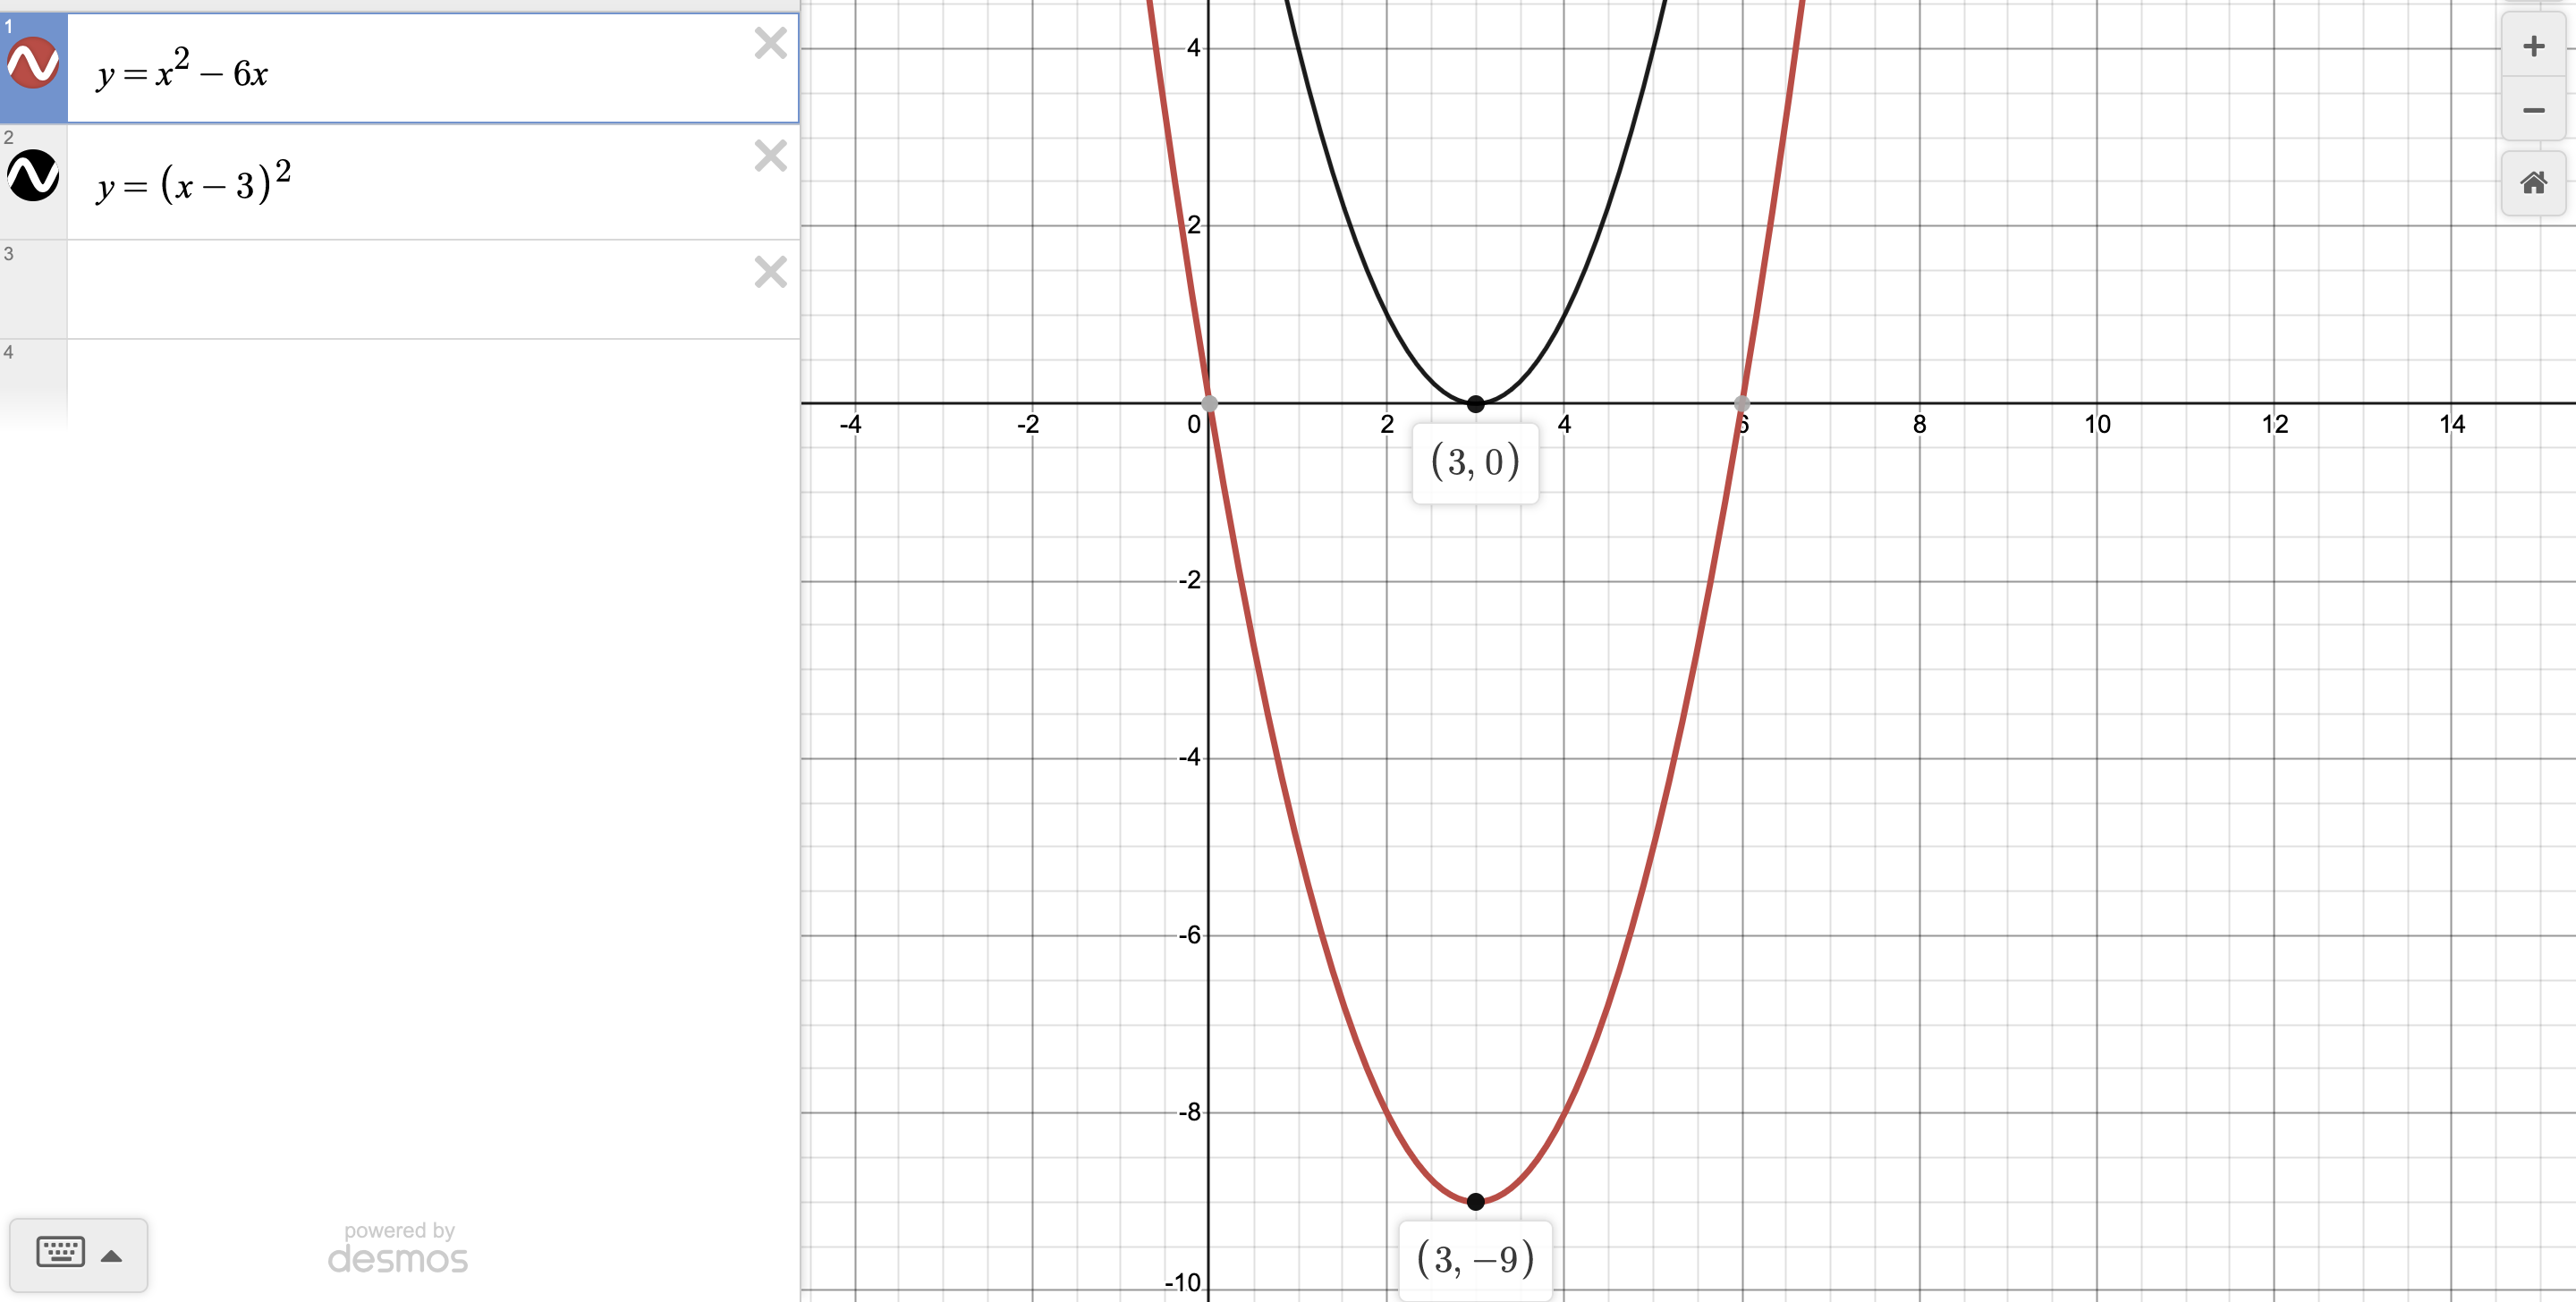
\includegraphics[width = 4in, height = 4in]{screenshot2}
\newline 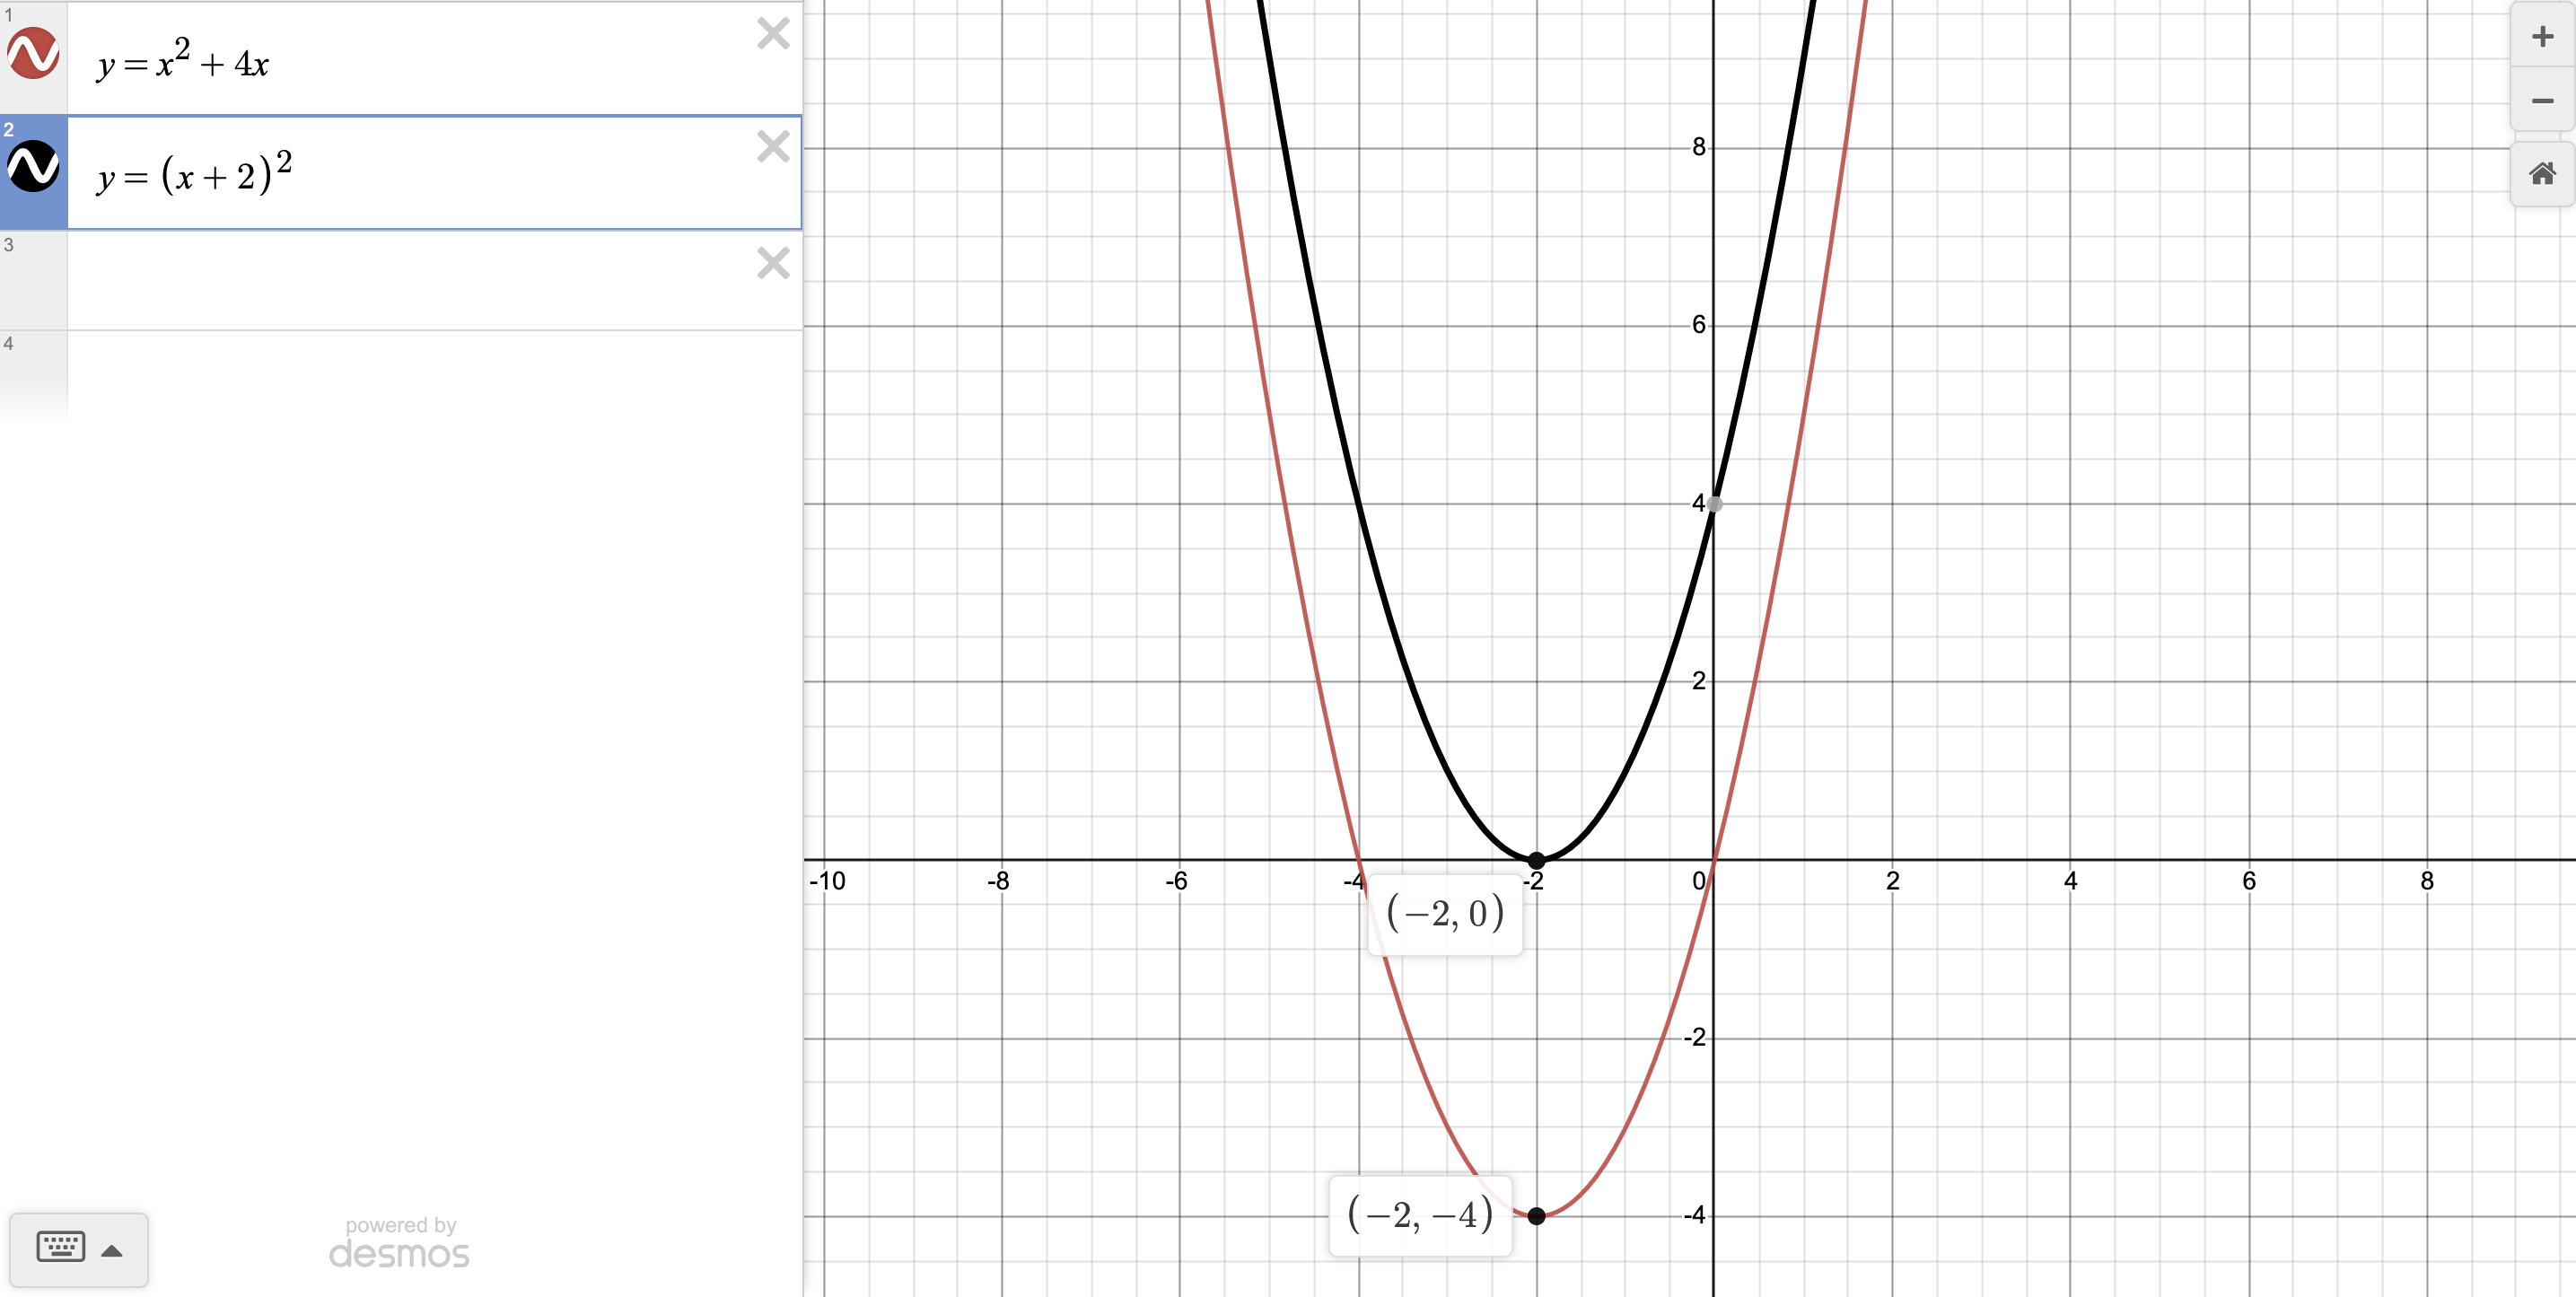
\includegraphics[width = 4in, height = 4in]{screenshot3}
\newline 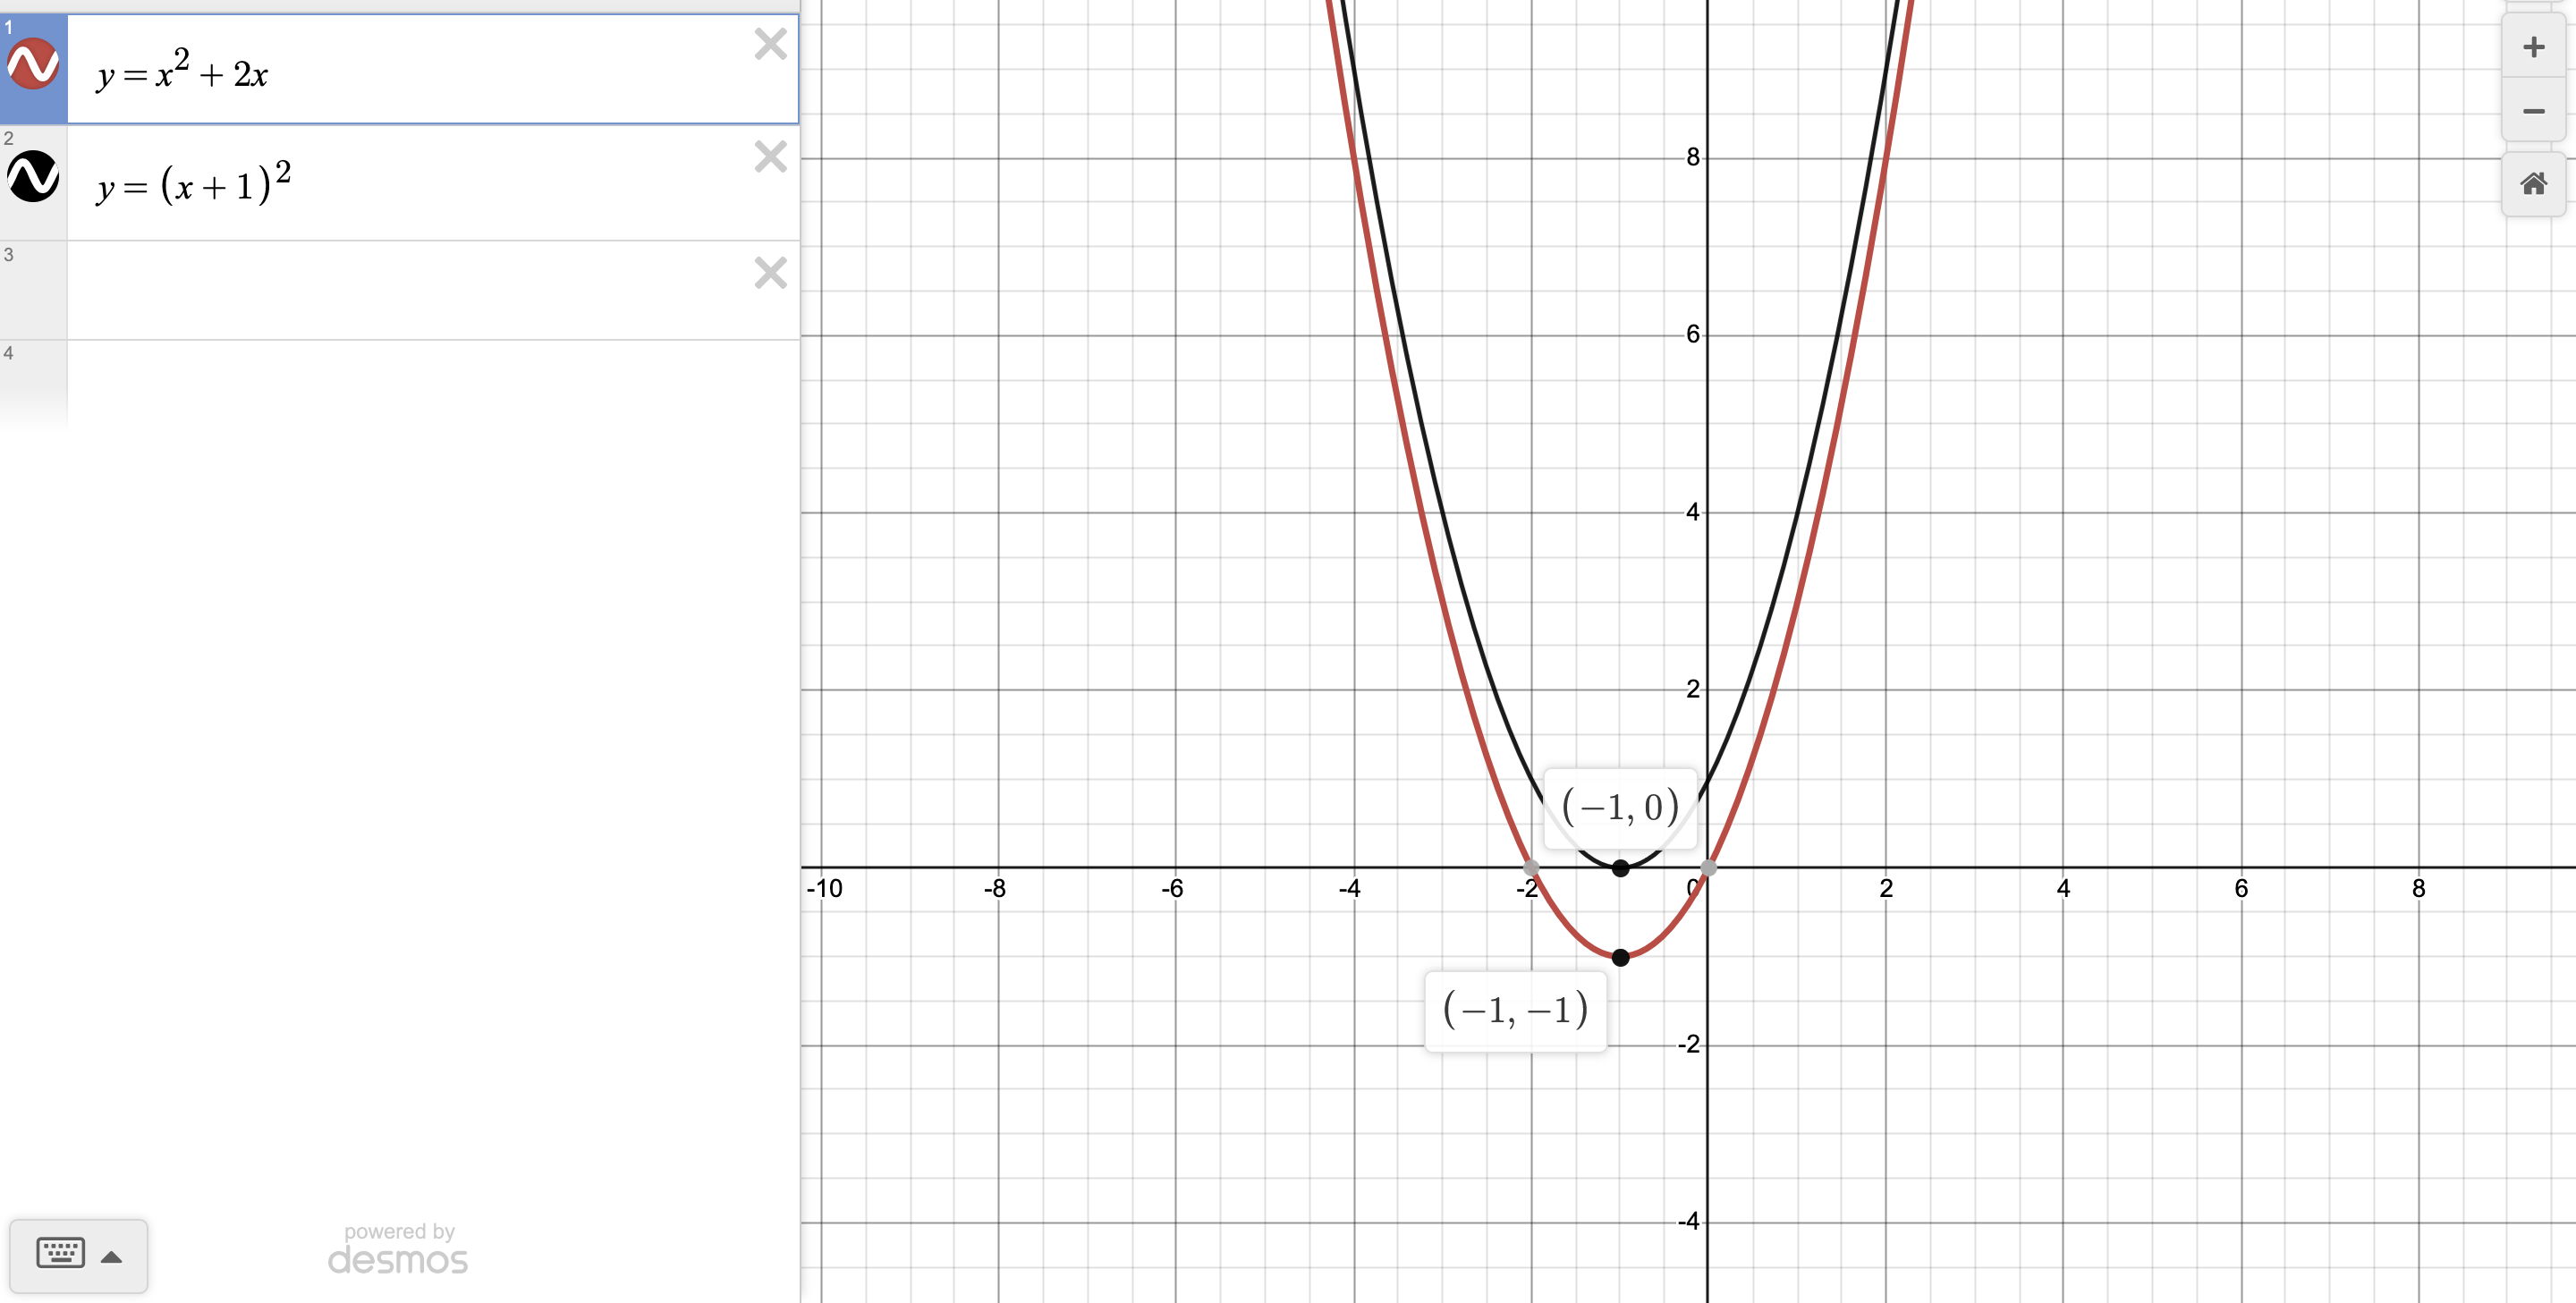
\includegraphics[width = 4in, height = 4in]{screenshot4}
(b):\newline In all the graphs, the $x$-coordinates of the two graphs in each pair are the same. However, in all of these graphs, the $y$-coordinate of the vertex changes 
to $-\frac{b}{2}^2$.
This noticeable pattern between these graphs suggests that changing the graph from $y=x^2+bx$ to $y=(x+\frac{b}{2})^2$ preserves the $x$-coordinate of the 
vertex, but changes the $y$ coordinate of the vertex to $-\frac{b}{2}^2$.


\section*{60}
We are given a quadratic equation in a form such that the left hand side of the equation can be factored into $(x+\frac{b}{2})^2$. Well, the only way 
a square root of a number has only one real solution is if that number is $0$. Hence, the only time there is one real solution is if $k=0$, with a solution 
of $x=-\frac{b}{2}+0=-\frac{b}{2}$. Whenever $x$ is a positive number, it follows that the square roots of $k$ are both real, and thus, the given 
equation has $2$ real solution iff $k>0$. With similar reasoning to the above, we can conclude that the given equation has two imaginary solutions iff $k<0$,
 because a number has two imaginary solutions iff it is a negative number. 


\section*{61}
$x^2+bx+c=0\newline\rightarrow x^2+bx=-c\newline\rightarrow x^2+bx+\frac{b}{2}^2=-c+\frac{b}{2}^2\newline\rightarrow 
(x+\frac{b}{2})^2=\frac{b^2-4c}{4}\newline\rightarrow x+\frac{b}{2}=\pm\frac{\sqrt{b^2-4c}}{\sqrt{4}}\newline\rightarrow 
x+\frac{b}{2}=\pm\frac{\sqrt{b^2-4c}}{2}\newline\rightarrow =-\frac{b}{2}\pm\frac{\sqrt{b^2-4c}}{2}\newline\rightarrow =\frac{-b\pm \sqrt{b^2-4c}}{2}$

\section*{62}
We can solve this problem by completing the square on the quadratic equation, in order to turn it into vertex form, thus giving us  
the maximum height:\newline $h=-16t^2+32t+6\newline\rightarrow h=-16(t^2-2t)+6\newline\rightarrow h-16=-16(t^2-2t+1)+6\newline\rightarrow 
h-16=-16(t-1)^2+6\newline\rightarrow h=-16(t-1)^2+22$, and thus, the vertex is $(1,22)$, meaning the maximum height is $22$ ft.

\section*{63}
We can solve this problem like the last one, converting it into vertex frm in order to find the maximum height:\newline
$h=-16t^2+48t+4\newline\rightarrow h=-16(t^2-3t)+4\newline\rightarrow h-36=-16(t^2-3t+2.25)+4\newline\rightarrow h=-16(t-1.5)^2+40$, and thus, 
the vertex is $(1.5,40)$, meaning the maximum height is $40$ ft.

\section*{64}
$y=(70-x)(50+x)\newline\rightarrow y=-x^2+20x+3500\newline\rightarrow y=-(x^2-20x)+3500\newline\rightarrow y-100=-(x^2-20x+100)+3500\newline\rightarrow 
y=-(x-10)^2+3600$, and thus, the vertex is $(10,3600)$, meaning the shop should sell 
skatesboards for $70-10=\$60$ to maximize weakly revenue at $\$3600$. 

\section*{65}
$y=(200+10x)(40-x)\newline\rightarrow =-10x^2+200x+8000\newline\rightarrow =-10(x^2-20x)+8000\newline\rightarrow y-1000=-10(x^2-20x+100)+8000\newline
\rightarrow y=-10(x-10)^2+9000$, and thus, the vertex is $(10,9000)$, meaning the shop should sell systems for $\$300$ to maximize revenue at 
$\$9000$.

\section*{66}
(a): $y=-0.0110x^2+1.23x+5.50\newline\rightarrow y=-0.0110(x^2-111.818)+5.50\newline\rightarrow y-34.384=-0.0110(x^2-111.818+3125.826)+5.50\newline
\rightarrow y=-0.0110(x-55.909)^2+39.884$\newline
(b): 
\begin{table}[h!]
        \begin{center}
                \begin{tabular}{l|c|c|c|c|c|c|c|c|c|c|r}
                        $x$ & $0$ & $10$ & $20$ & $30$ & $40$ & $50$ & $60$ & $70$ & $80$ & $90$ & $100$\\
                        \hline
                        $y$ & $5.5$ & $16.656$ & $25.656$ & $32.456$ & $37.056$ & $39.456$ & $39.656$ & $37.656$ & $33.456$ & $27.056$ & $18.456$
                \end{tabular}
        \end{center}
\end{table}
\begin{table}[h!]
        \begin{center}
                \begin{tabular}{l|c|r}
			$x$ & $110$ & $120$\\
                        \hline
			$y$ & $7.656$ & $-5.344$
                \end{tabular}
        \end{center}
\end{table}
\newline (c): 
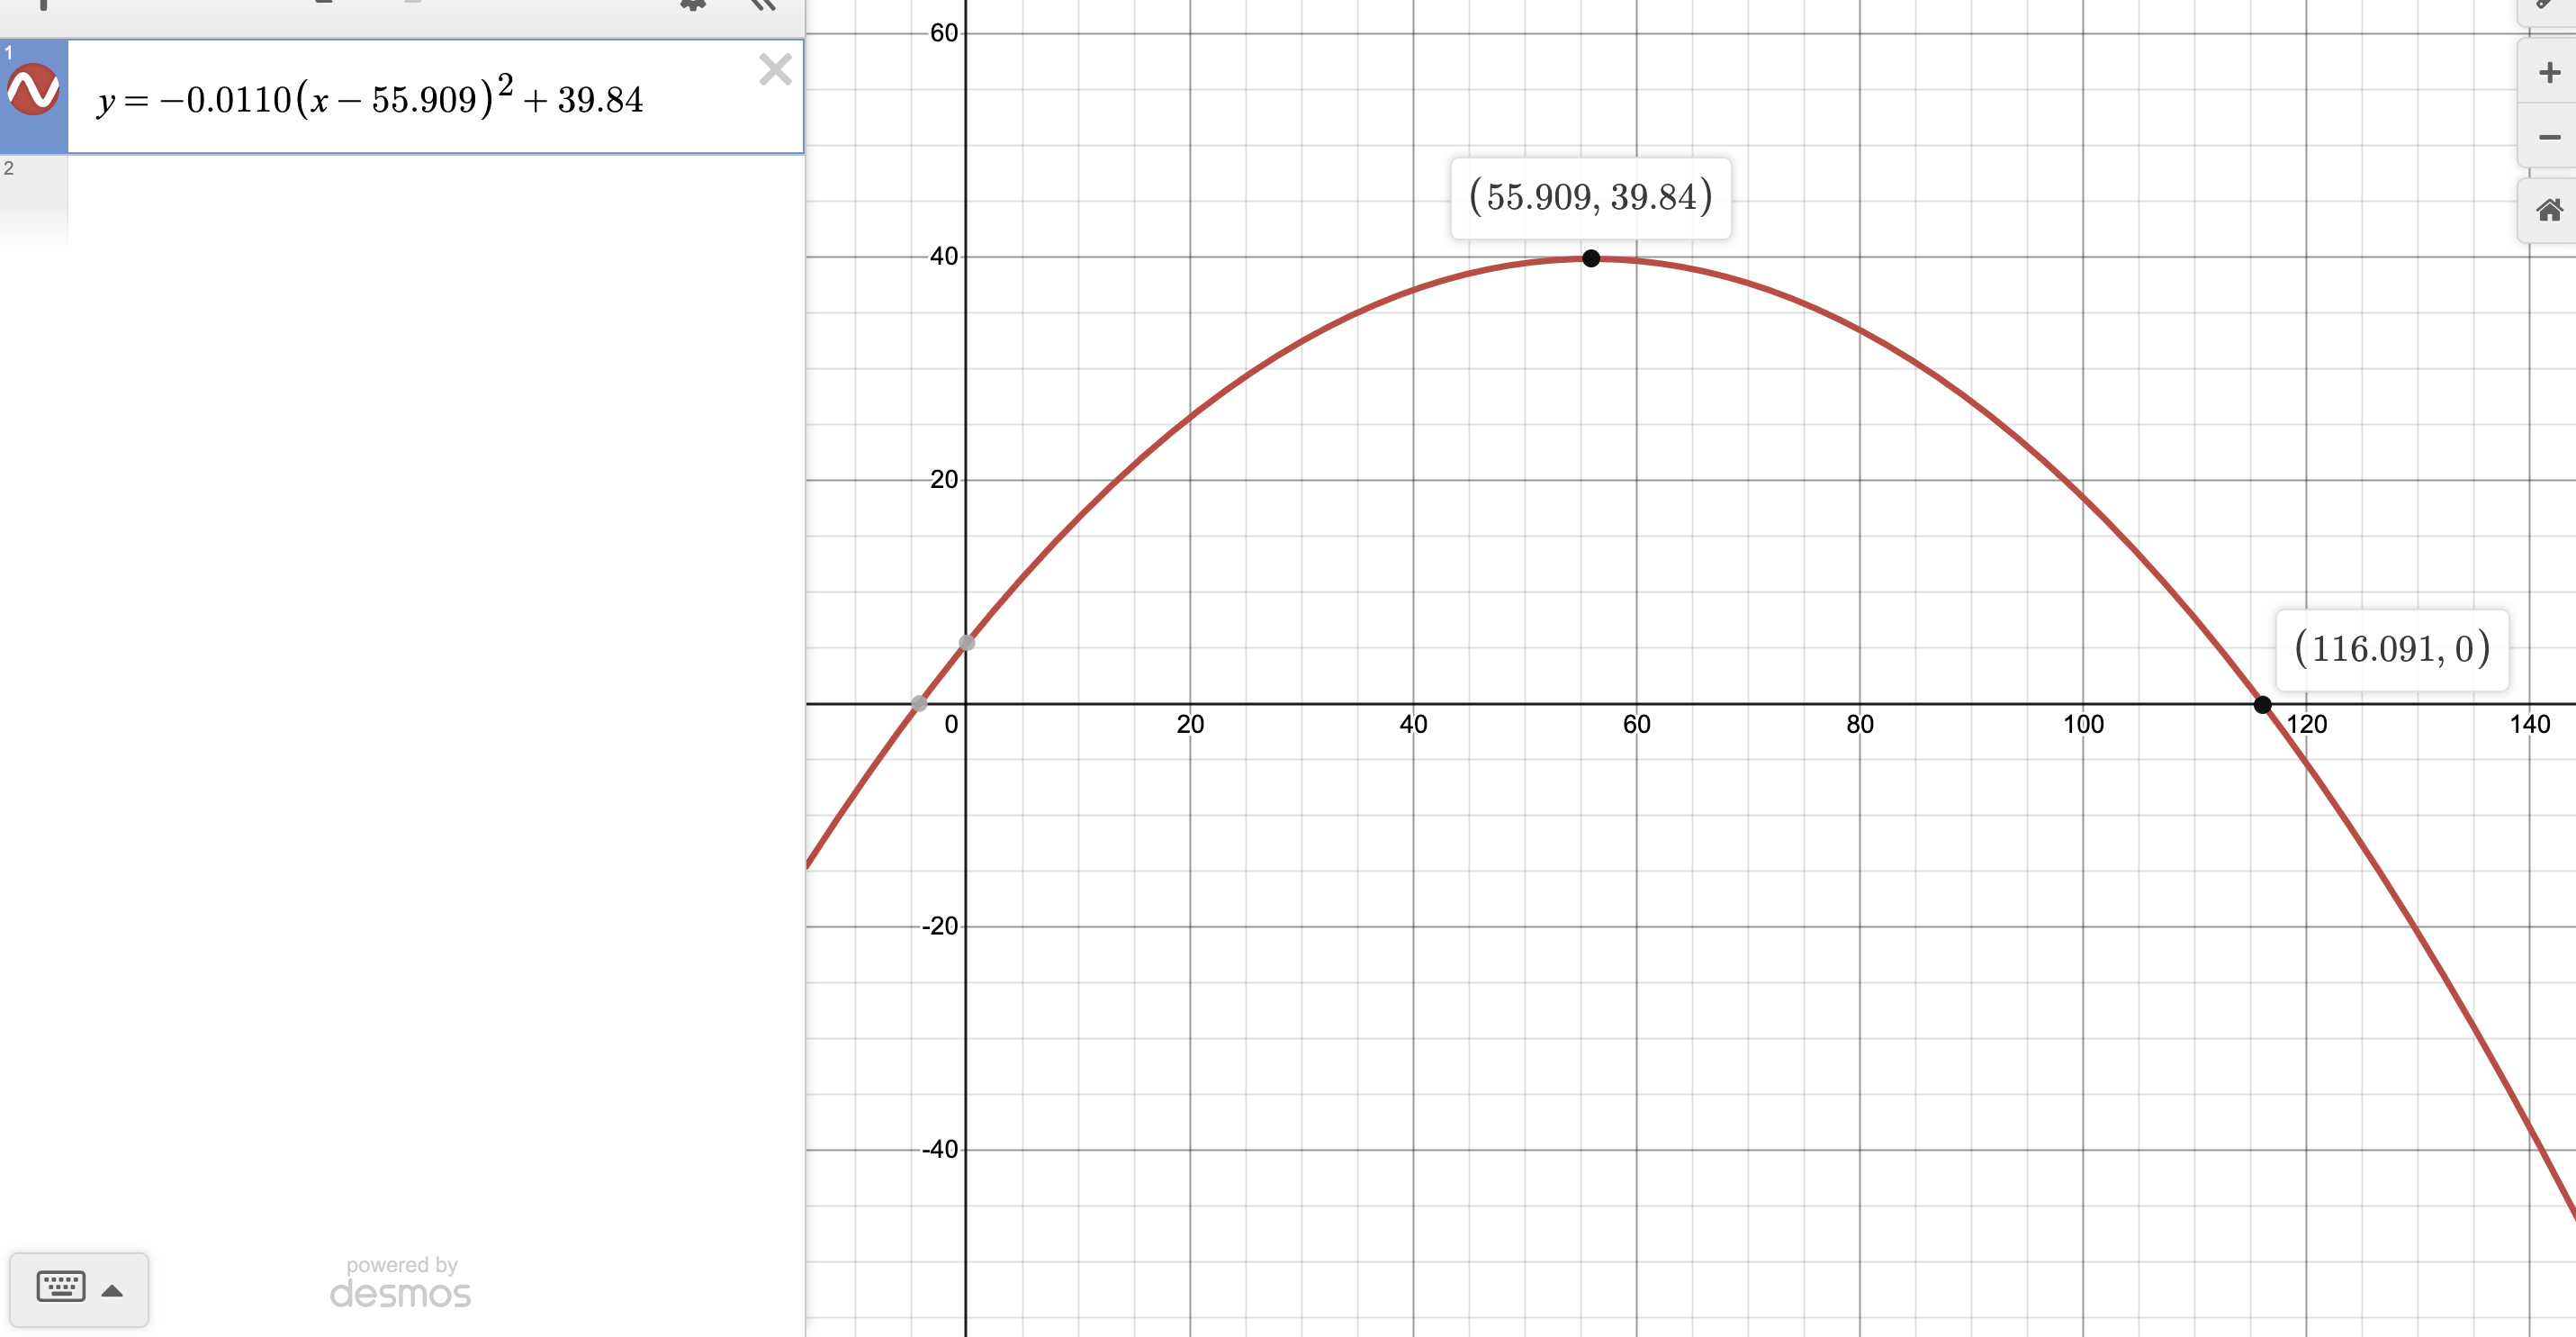
\includegraphics[width = 4in, height = 4in]{secondscreenshot}
Thus, we can see that the softball reaches a maximum height of $\approx 39.84$ ft., and travels a total distance of $\approx 116.091$ ft.

\section*{67}
(a): A verbal model for this equation is $Total\ Area=Width\times Length$, and hence, we recieve:\newline $1500=(120-2x)(x)$.\newline
(b): $(120-2x)x=1500\newline\rightarrow -2x^2+120x=1500\newline\rightarrow x^2-60x=-750\newline\rightarrow x^2-60x+900=150\newline\rightarrow 
(x-30)^2=150\newline\rightarrow x=30\pm 5\sqrt{6}$ Well, if $x=30-5\sqrt{6}$, then the width of the enclosure would be $120-2(30-5\sqrt{6})\approx 85.5$, 
which is greater than the given fact that the siding of this enclosure cannot be greater than the side of the school, and hence, this possibilty is ruled 
out. Thus, $x=30+5\sqrt{6}$.\newline
(c): The dimesnions of the part of this section parallel to the wall
 are $120-2(30+5\sqrt{6})\approx 35.5$ ft., while the dimesnions of the other part of this section is $30+5\sqrt{6}\approx 42.2$ ft.

\section*{68}
To solve this question, we need to find $x$, the thickness of the pencilholder. We are given the radius of the smaller cylinder, as well as the height, meaning the 
volume of the smaller cylinder is $\pi 3^2\times 9\pi(9-x)$. 
We also know that the total volume of clay, $200$ cubic centimeters, equals the difference of the volumes 
of the two cylinders. This allows us to set up an equation that can let us find the radius of the entire cylinder, as shown below:\newline 
$200=9\pi(3+x)^2-9\pi(9-x)\newline\rightarrow
200=9\pi((3+x)^2-(9-x))\newline\rightarrow
200=9\pi x^2+63\pi x\newline\rightarrow 
9\pi x^2+63\pi x-200=0\newline\rightarrow
x=\frac{-63\pi\pm\sqrt{63\pi ^2-4(9\pi)(-200)}}{2(9\pi)}\newline\rightarrow 
x=\frac{-63\pi\pm\sqrt{63\pi ^2+7200\pi}}{2(9\pi)}\newline\rightarrow 
x=0.896\vee x=-446.500$ and thus, because only positive values are accepted, the thickness $x$ that the pencil holder should have is $0.896$ centimeters. 



\end{document}
